\documentclass[11pt,a4paper]{article}

% ── Packages ────────────────────────────────────────────────────────────────
\usepackage[margin=2.5cm]{geometry}
\usepackage{amsmath,amssymb,amsthm}
\usepackage{booktabs}
\usepackage{array}
\usepackage{tabularx}
\usepackage{multirow}
\usepackage{graphicx}
\usepackage{xcolor}
\usepackage{hyperref}
\usepackage{algorithm}
\usepackage{algpseudocode}
\usepackage{tikz}
\usetikzlibrary{shapes.geometric, arrows.meta, positioning, fit, backgrounds}
\usepackage{caption}
\usepackage{subcaption}
\usepackage{enumitem}
\usepackage{mathtools}
\usepackage{microtype}
\usepackage{parskip}
\usepackage{fancyhdr}
\usepackage{titlesec}
\usepackage{tcolorbox}
\tcbuselibrary{skins,breakable}

% ── Colours ─────────────────────────────────────────────────────────────────
\definecolor{accentblue}{RGB}{30,90,160}
\definecolor{lightblue}{RGB}{220,235,255}
\definecolor{accentgreen}{RGB}{30,130,80}
\definecolor{lightgreen}{RGB}{220,250,235}
\definecolor{accentred}{RGB}{180,40,40}
\definecolor{lightgrey}{RGB}{248,248,248}
\definecolor{darkgrey}{RGB}{80,80,80}

% ── Hyperref ────────────────────────────────────────────────────────────────
\hypersetup{
  colorlinks=true,
  linkcolor=accentblue,
  urlcolor=accentblue,
  citecolor=accentblue,
  pdftitle={Model Instability Under Minority Data Scarcity},
  pdfauthor={Research Proposal},
}

% ── Headers ─────────────────────────────────────────────────────────────────
\pagestyle{fancy}
\fancyhf{}
\fancyhead[L]{\small\color{darkgrey}Model Instability Under Minority Data Scarcity}
\fancyhead[R]{\small\color{darkgrey}Research Pitch}
\fancyfoot[C]{\thepage}
\renewcommand{\headrulewidth}{0.4pt}

% ── Section styling ─────────────────────────────────────────────────────────
\titleformat{\section}{\large\bfseries\color{accentblue}}{}{0em}{\thesection\quad}[\vspace{-0.3em}\hrule\vspace{0.2em}]
\titleformat{\subsection}{\normalsize\bfseries\color{accentblue}}{\thesubsection}{1em}{}

% ── Custom boxes ────────────────────────────────────────────────────────────
\newtcolorbox{framebox}[2][]{
  colback=lightblue, colframe=accentblue,
  fonttitle=\bfseries, title=#2, #1,
  breakable
}
\newtcolorbox{claimbox}[1][]{
  colback=lightgreen, colframe=accentgreen,
  fonttitle=\bfseries, #1,
  breakable
}

% ── Algorithm style ─────────────────────────────────────────────────────────
\algrenewcommand\algorithmicindent{1.2em}

% ── Macros ──────────────────────────────────────────────────────────────────
\newcommand{\Dplus}{D^{+}}
\newcommand{\Dminus}{D^{-}}
\newcommand{\Dbnd}{D^{+}_{\mathrm{bnd}}}
\newcommand{\Dsafe}{D^{+}_{\mathrm{safe}}}
\newcommand{\Daug}{D_{\mathrm{aug}}}
\newcommand{\Dval}{D_{\mathrm{val}}}
\newcommand{\Pf}{P_{f_0}}
\newcommand{\IR}{\mathrm{IR}}
\newcommand{\CV}{\mathrm{CV}}

% ════════════════════════════════════════════════════════════════════════════
\begin{document}

% ── Title block ─────────────────────────────────────────────────────────────
\begin{titlepage}
\centering
\vspace*{2cm}
{\small\color{darkgrey}\scshape Research Pitch $\mid$ Empirical Study\par}
\vspace{0.8cm}
{\LARGE\bfseries\color{accentblue} Model Instability Under Minority Data Scarcity\par}
\vspace{0.5cm}
{\Large An Empirical Study of Model Capacity in Imbalanced Classification\par}
\vspace{1.2cm}
\hrule height 1.5pt
\vspace{0.4cm}
{\large A structured research roadmap covering datasets, models, metrics,\\
existing baselines, and the proposed \textbf{AMBA} framework\par}
\vspace{0.4cm}
\hrule height 0.5pt
\vspace{2cm}
\begin{tabular}{ll}
\textbf{Status:} & Research Proposal / Pitch \\[4pt]
\textbf{Date:}   & 2026 \\
\end{tabular}
\vfill
\end{titlepage}

% ── Abstract ────────────────────────────────────────────────────────────────
\begin{abstract}
\noindent
Class imbalance---the condition where one class vastly outnumbers another---is one of the
most common and consequential obstacles in applied machine learning. Real-world high-stakes
tasks, including fraud detection, rare disease diagnosis, and network intrusion identification,
suffer from severe imbalance. Existing work predominantly reports average performance
improvements under standard resampling or cost-sensitive methods, without closely examining
the \emph{stability} of model predictions across experimental runs, data splits, and varying
imbalance ratios.

This document pitches a structured empirical study with three goals. First, we benchmark
seven commonly used classifiers across four carefully chosen datasets spanning a wide range
of imbalance intensities, using both performance and stability metrics. Second, we apply a
representative set of existing imbalance-handling techniques as baselines. Third, we introduce
\textbf{AMBA} (\textbf{A}daptive \textbf{M}inority \textbf{B}oundary \textbf{A}ugmentation)---a
novel framework that combines imbalance-ratio-aware routing, uncertainty-guided synthetic
oversampling with a scarcity-proportional budget, and stability-weighted ensemble
aggregation. AMBA is designed from the ground up to address prediction instability that
existing techniques overlook, while explicitly adapting its strategy to the imbalance severity
and separability of the data.

\noindent\textit{No experimental results are reported in this document; the goal is to establish
the research question, motivate the experimental choices, and describe the proposed
methodology with sufficient mathematical and algorithmic precision to serve as a working
blueprint.}
\end{abstract}

\tableofcontents
\newpage

% ════════════════════════════════════════════════════════════════════════════
\section{Introduction and Motivation}

In many real-world classification tasks, the distribution of class labels is far from uniform.
A dataset used to detect fraudulent credit card transactions may contain 99.8\,\% legitimate
records and only 0.2\,\% fraud. A medical screening dataset may contain 95\,\% healthy
patients and 5\,\% at-risk individuals. This asymmetry---called \emph{class imbalance}---
creates a fundamental challenge: a naive classifier that always predicts the majority class can
achieve very high accuracy while being completely useless in practice.

\subsection{Why Instability Is the Overlooked Problem}

The machine learning community has responded to class imbalance with a large toolkit:
oversampling, undersampling, cost-sensitive learning, and ensemble methods. Most benchmark
studies report that these techniques improve the mean F1-score or AUC-ROC over a baseline.
However, three important questions are rarely asked:

\begin{enumerate}
  \item Does the performance improvement come with \emph{consistent} results, or does the
        improved mean hide high variance across folds and runs?
  \item Do different classifier architectures behave differently in terms of stability when
        minority data is scarce?
  \item Can we deliberately engineer a method that optimises \emph{both} the level and the
        stability of minority-class performance, while adapting its strategy to the regime of
        imbalance it encounters?
\end{enumerate}

\begin{claimbox}
\textbf{Central Claim.} A technique that achieves a slightly lower mean F1-score but with
half the variance is often more operationally useful than a technique with a higher mean but
unpredictable individual-run behaviour. We argue that stability is a first-class evaluation
criterion, not an afterthought---and that an effective imbalance-handling framework must
adapt its augmentation strategy to the structure of the data it receives.
\end{claimbox}

\subsection{Scope of This Study}

We restrict ourselves to tabular, binary classification problems. This scope is chosen
deliberately: tabular data remains the dominant form in industry, binary classification is the
clearest setting for studying minority-class behaviour, and it avoids confounds from
domain-specific representation learning (e.g., image or text encoders).

% ════════════════════════════════════════════════════════════════════════════
\section{Problem Formulation}

\subsection{Formal Setup}

Let $\mathcal{D} = \{(\mathbf{x}_i, y_i)\}_{i=1}^{N}$ be a labelled dataset where
$\mathbf{x}_i \in \mathbb{R}^d$ is a feature vector and $y_i \in \{0,1\}$ is the class label.
We denote the majority class as $y=0$ and the minority class as $y=1$. Define:
\[
  \Dplus = \{(\mathbf{x}_i, y_i) \mid y_i = 1\}, \qquad
  \Dminus = \{(\mathbf{x}_i, y_i) \mid y_i = 0\}.
\]
The \emph{Imbalance Ratio} is:
\[
  \IR = \frac{|\Dminus|}{|\Dplus|}.
\]
A dataset is considered \emph{mildly} imbalanced if $\IR < 5$, \emph{moderately} imbalanced
if $\IR \in [5, 50]$, and \emph{severely} or \emph{extremely} imbalanced if $\IR > 100$.

\subsection{The Learning Objective Under Imbalance}

A standard classifier minimises the empirical risk:
\[
  \hat{f} = \arg\min_{f \in \mathcal{F}} \frac{1}{N} \sum_{i=1}^{N}
  \ell\!\bigl(f(\mathbf{x}_i),\, y_i\bigr),
\]
where $\ell$ is a loss function. Under standard 0-1 loss and high imbalance, this optimisation
is biased toward the majority class because majority errors dominate the sum. As a result,
$\hat{f}$ tends to underperform on $\Dplus$.

\subsection{Defining Stability}

Let $\mathcal{S} = \{S_1, S_2, \ldots, S_K\}$ be a set of cross-validation folds. Let $m_k$
be a performance metric (e.g., recall or F1-score on the minority class) computed on fold $k$.
We define the fold mean and standard deviation:
\[
  \bar{m} = \frac{1}{K}\sum_{k=1}^{K} m_k, \qquad
  \sigma_m = \sqrt{\frac{1}{K-1}\sum_{k=1}^{K}(m_k - \bar{m})^2}.
\]
The \emph{Coefficient of Variation} (CV) is:
\[
  \CV(m) = \frac{\sigma_m}{\bar{m}}.
\]
A lower CV indicates greater stability. Our study will report both $\bar{m}$ and $\CV(m)$
for all model--technique combinations.

% ════════════════════════════════════════════════════════════════════════════
\section{Candidate Datasets}

We select four publicly available binary classification datasets spanning a wide spectrum of
imbalance ratios, sample sizes, and application domains. This diversity is intentional: a good
technique should generalise across settings.

\begin{table}[ht]
\centering
\caption{Summary of candidate datasets ordered by increasing imbalance ratio.}
\begin{tabular}{lrrrll}
\toprule
\textbf{Dataset} & \textbf{$N$} & \textbf{Features} & \textbf{IR} & \textbf{Category} & \textbf{Domain} \\
\midrule
Pima Indians Diabetes    &    768 &  8 & $\approx 1.9$ & Mild     & Biomedical      \\
Sick (Thyroid Disease{,} OpenML)    &  3{,}772 & 29 & $\approx 15$  & Moderate & Medical         \\
Mammography (OpenML)     & 11{,}183 &  6 & $\approx 42$  & High     & Medical Imaging \\
Credit Card Fraud (ULB)  & 284{,}807 & 30 & $\approx 578$ & Extreme  & Finance         \\
\bottomrule
\end{tabular}
\end{table}

\subsection{Dataset Descriptions}

\textbf{1.~Pima Indians Diabetes ($\IR \approx 1.9$).} Sourced from the UCI Machine
Learning Repository, this dataset records eight clinical measurements from Pima Indian women
alongside a binary diabetes indicator. With mild imbalance it serves as the near-baseline
condition, showing model behaviour before minority scarcity becomes severe.

\textbf{2.~Sick Dataset ($\IR \approx 15$).}  Clinical thyroid screening dataset with multiple laboratory and diagnostic features, reduced to a binary classification problem. The moderate imbalance and relatively large sample size make it well-suited for studying model stability and performance under intermediate skew, bridging the gap between near-balanced and highly imbalanced regimes.

\textbf{3.~Mammography Dataset ($\IR \approx 42$).} Available on OpenML (dataset ID 310),
this records pixel features from mammography scans with malignancy as the minority class.
The high IR and small minority count ($\approx 260$ samples) make it a realistic test of
techniques under genuine data scarcity.

\textbf{4.~Credit Card Fraud Detection ($\IR \approx 578$).} Released by the ULB Machine
Learning Group, this contains transaction-level features from European cardholders with 492
fraud cases in 284{,}807 total transactions. The extreme imbalance and large scale make it
the hardest dataset in our suite.

% ════════════════════════════════════════════════════════════════════════════
\section{Candidate Models}

We select seven classifiers spanning a wide range of inductive biases, capacities, and
decision-boundary geometries. This diversity is necessary to study how model type interacts
with imbalance and with different remediation techniques.

\begin{table}[ht]
\centering
\caption{Summary of the seven candidate models.}
\begin{tabularx}{\textwidth}{llX}
\toprule
\textbf{ID} & \textbf{Model} & \textbf{Rationale for Inclusion} \\
\midrule
M1 & Logistic Regression (LR)       & Linear boundary; well-calibrated probabilities; directly sensitive to class priors \\
M2 & Support Vector Machine (SVM, RBF) & Margin-based; implicit regularisation; known to struggle with severe imbalance \\
M3 & Decision Tree (DT)             & Axis-aligned boundaries; prone to majority-dominated splits \\
M4 & Random Forest (RF)             & Ensemble of trees; partial robustness through bagging \\
M5 & Gradient Boosted Trees (XGBoost) & Sequential boosting; supports controllable class weights \\
M6 & Multi-layer Perceptron (MLP)   & Flexible non-linear model; highly sensitive to minority sample count \\
M7 & K-Nearest Neighbours (KNN)     & Non-parametric; directly affected by neighbourhood density imbalance \\
\bottomrule
\end{tabularx}
\end{table}

% ════════════════════════════════════════════════════════════════════════════
\section{Evaluation Metrics}

\subsection{Why Accuracy Alone Fails}

On a dataset with $\IR = 100$:$1$, a classifier that always predicts the majority class
achieves 99\,\% accuracy. This makes standard accuracy an unreliable metric under imbalance;
we require metrics sensitive to minority-class performance.

\subsection{Confusion Matrix Foundations}

For binary classification, the confusion matrix defines four counts: True Positives (TP),
True Negatives (TN), False Positives (FP), and False Negatives (FN). Under imbalance,
FN (missed minority samples) is typically the most costly error.

\subsection{Performance Metrics}

\begin{align}
  \text{Precision} &= \frac{\mathrm{TP}}{\mathrm{TP}+\mathrm{FP}} \label{eq:prec}\\[4pt]
  \text{Recall} &= \frac{\mathrm{TP}}{\mathrm{TP}+\mathrm{FN}} \label{eq:rec}\\[4pt]
  \text{F1-score} &= \frac{2\cdot\text{Precision}\cdot\text{Recall}}{\text{Precision}+\text{Recall}}
                 = \frac{2\,\mathrm{TP}}{2\,\mathrm{TP}+\mathrm{FP}+\mathrm{FN}} \label{eq:f1}\\[4pt]
  \text{AUC-ROC} &= \int_0^1 \mathrm{TPR}(t)\,\mathrm{d}\,\mathrm{FPR}(t) \label{eq:auc}\\[4pt]
  \text{G-Mean} &= \sqrt{\text{Sensitivity}\times\text{Specificity}}
                = \sqrt{\frac{\mathrm{TP}}{\mathrm{TP}+\mathrm{FN}}\cdot\frac{\mathrm{TN}}{\mathrm{TN}+\mathrm{FP}}}
                \label{eq:gmean}\\[4pt]
  \text{MCC} &= \frac{\mathrm{TP}\cdot\mathrm{TN}-\mathrm{FP}\cdot\mathrm{FN}}
               {\sqrt{(\mathrm{TP}+\mathrm{FP})(\mathrm{TP}+\mathrm{FN})(\mathrm{TN}+\mathrm{FP})(\mathrm{TN}+\mathrm{FN})}}
               \label{eq:mcc}
\end{align}

\textit{Note on MCC.} Matthews Correlation Coefficient considers all four confusion matrix
cells and is invariant to class prevalence. Its range is $[-1,+1]$, where $+1$ is perfect,
$0$ is no better than random, and $-1$ is perfectly wrong.

\subsection{Stability Metrics}

In addition to point-estimate performance metrics, we report the following stability quantities
computed over $K$-fold cross-validation:
\begin{align}
  \CV(\text{F1}) &= \frac{\sigma_{\text{F1}}}{\bar{F}_1}
                  \quad\text{(Coefficient of Variation of F1)} \label{eq:cvf1}\\[4pt]
  \CV(\text{Recall}) &= \frac{\sigma_{\text{Recall}}}{\overline{\text{Recall}}} \label{eq:cvrec}\\[4pt]
  \mathrm{IQR}(m) &= Q_{75}(m) - Q_{25}(m)
                   \quad\text{(Interquartile Range of metric }m\text{)} \label{eq:iqr}
\end{align}

\begin{table}[ht]
\centering
\caption{Complete metric suite. The left block measures performance level; the right block
measures consistency across folds.}
\begin{tabular}{llll|llll}
\toprule
\multicolumn{4}{c|}{\textbf{Performance Metrics}} & \multicolumn{4}{c}{\textbf{Stability Metrics}} \\
\midrule
Metric     & Summary               & Goal & & Metric         & Measures          & Goal & \\
\midrule
Precision  & TP/(TP+FP)            & $\uparrow 1$ & & CV(F1)     & F1 consistency    & $\downarrow 0$ & \\
Recall     & TP/(TP+FN)            & $\uparrow 1$ & & CV(Recall) & Recall consistency& $\downarrow 0$ & \\
F1-score   & Harmonic mean (P, R)  & $\uparrow 1$ & & $\sigma$(MCC) & MCC spread     & $\downarrow 0$ & \\
AUC-ROC    & Area under ROC        & $\uparrow 1$ & & IQR(F1)    & Fold robustness   & $\downarrow 0$ & \\
G-Mean     & $\sqrt{\text{Sens}\times\text{Spec}}$ & $\uparrow 1$ & & & & & \\
MCC        & Balanced correlation  & $\uparrow 1$ & & & & & \\
\bottomrule
\end{tabular}
\end{table}

% ════════════════════════════════════════════════════════════════════════════
\section{Existing Imbalance-Handling Techniques (Baselines)}

We organise existing techniques into three families. Each will be applied to each of the seven
models across all four datasets, yielding a comprehensive baseline surface for comparison.

\subsection{Data-Level Techniques}

\textbf{Random Oversampling.} Minority samples are duplicated uniformly at random until a
target ratio is reached.

\textbf{Random Undersampling.} Majority samples are removed uniformly at random to reduce
the imbalance, at the risk of discarding useful majority-class information.

\textbf{SMOTE.} For each $\mathbf{x}_i \in \Dplus$, SMOTE finds its $k$ nearest minority
neighbours and generates a synthetic sample by linear interpolation:
\[
  \mathbf{x}_{\mathrm{syn}} = \mathbf{x}_i + \lambda\,(\mathbf{x}_{\mathrm{nn}} - \mathbf{x}_i),
  \quad \lambda \sim \mathcal{U}[0,1].
\]

\textbf{ADASYN.} Generates more samples for harder minority instances. The difficulty of
$\mathbf{x}_i$ is proportional to the number of majority neighbours in its $k$-neighbourhood:
\[
  r_i = \frac{\Delta_i}{k}, \qquad \hat{r}_i = \frac{r_i}{\sum_j r_j}.
\]

\textbf{Tomek Links.} A cross-class pair $(\mathbf{x}_i, \mathbf{x}_j)$ is a Tomek Link if
each is the other's nearest neighbour. Removing the majority-class member from each link
cleans the decision boundary region.

\subsection{Algorithm-Level Techniques}

\textbf{Class Weighting.} The loss is scaled to penalise minority errors more heavily:
\[
  \ell_w(\hat{y}, y) = w_y \cdot \ell(\hat{y}, y), \quad
  w_1 = \frac{N}{2|\Dplus|}, \quad w_0 = \frac{N}{2|\Dminus|}.
\]

\textbf{Threshold Moving.} Rather than using the default 0.5 decision threshold, $\tau^*$ is
tuned on a validation set to maximise a target metric:
\[
  \hat{y} = \mathbf{1}\!\bigl[P(y=1\mid\mathbf{x}) \ge \tau^*\bigr], \quad
  \tau^* = \arg\max_\tau\, \mathrm{G\text{-}Mean}(\tau).
\]

\subsection{Ensemble-Level Techniques}

\textbf{Balanced Bagging.} Multiple classifiers are trained on bootstrapped subsets, each
balanced by undersampling the majority class to match the minority count.

\textbf{EasyEnsemble.} An ensemble of AdaBoost classifiers is trained on different random
majority-class undersamples, with final predictions by majority vote.

% ════════════════════════════════════════════════════════════════════════════
\section{Proposed Technique: AMBA}

\begin{framebox}{AMBA: Adaptive Minority Boundary Augmentation}
A four-component framework that (1) routes the pipeline according to the imbalance ratio
and baseline class separability; (2) uses an imbalance-adaptive initial classifier to locate
minority samples near the decision boundary; (3) generates synthetic samples in this boundary
region using gradient-directed interpolation within a scarcity-proportional budget; and (4)
aggregates an ensemble of classifiers weighted by their cross-validated stability rather than
their mean performance alone.
\end{framebox}

\subsection{Motivation}

Existing oversampling and ensemble methods share three key limitations:

\begin{enumerate}
  \item \textbf{Geometrically blind augmentation.} SMOTE generates synthetic samples
        uniformly in the minority neighbourhood without regard for where the decision boundary
        lies, potentially reinforcing already-covered regions while leaving the boundary zone
        sparse.
  \item \textbf{Ignoring instability as a design criterion.} No existing technique explicitly
        minimises prediction variance as part of its objective.
  \item \textbf{One-size-fits-all strategy.} Existing techniques apply the same augmentation
        logic regardless of the imbalance ratio or the intrinsic separability of the classes.
        At mild imbalance the minority class is already well-represented; heavy augmentation
        introduces noise. At extreme imbalance, unconstrained synthesis risks mode collapse.
        When classes are already well-separated, augmentation adds variance, not signal.
\end{enumerate}

AMBA addresses all three limitations through an adaptive routing system and a
scarcity-aware synthesis budget.

\subsection{Component 0: Adaptive Pre-Flight Routing}

Before entering the main pipeline, AMBA applies two routing checks.

\subsubsection*{IR-Adaptive Bypass (handles mild imbalance)}

\[
  \text{If } \IR < \tau_{\IR}: \quad
  \hat{y} = \mathbf{1}\!\bigl[P_f(y=1 \mid \mathbf{x}) \ge \tau^*\bigr],\;
  \tau^* = \arg\max_\tau \mathrm{G\text{-}Mean}(\tau, \Dval),
\]
where $f$ is a standard cross-validated classifier with no augmentation. At mild imbalance
($\IR < \tau_{\IR}$, default: 5) the minority class is naturally well-represented across folds.
The overhead of boundary detection, guided synthesis, and ensemble construction introduces
variance without benefit. Threshold Moving is the appropriate lightweight alternative here.

\subsubsection*{AUC-Gated Augmentation Bypass (handles near-perfectly separated classes)}

After a pilot 3-fold cross-validation on the raw data, compute the mean baseline AUC. If
$\mathrm{AUC}_{\mathrm{baseline}} \ge \theta_{\mathrm{AUC}}$ (default: 0.97), skip Stages 1
and 2 (no synthetic oversampling) and execute Stage 3 only: train the stability-weighted
ensemble on the raw class-weighted data. This retains the stability benefit of ensemble
weighting while avoiding the noise from augmenting an already-solved classification problem.

When the baseline AUC exceeds 0.97, the model has effectively learned the decision boundary.
Boundary-directed synthesis in Stage 2 would be solving a problem that does not exist.

\subsection{Stage 1: Adaptive Boundary Detection}

Train an initial classifier $f_0$ on the raw imbalanced data $\mathcal{D}$ using an
IR-conditioned selector:

\[
  f_0 = \begin{cases}
    \text{Logistic Regression} & \text{if } \IR < \tau_{f_0} \\
    \text{Random Forest (shallow, max\_depth = 4)} & \text{if } \IR \ge \tau_{f_0}
  \end{cases}
\]

with $\tau_{f_0}$ defaulting to 20. At high IR, the minority samples form a sparse, possibly
non-convex cluster that a linear boundary cannot fit. A shallow Random Forest captures
non-linear boundaries without overfitting and provides well-calibrated minority-class
probabilities after Platt scaling.

For each $\mathbf{x}_i \in \Dplus$, compute its boundary proximity score:
\[
  b_i = 1 - 2\Bigl|\Pf(y=1 \mid \mathbf{x}_i) - 0.5\Bigr| \in [0,1].
\]
$b_i \approx 1$ means $\mathbf{x}_i$ is near the boundary (the model is uncertain);
$b_i \approx 0$ means it lies well inside the minority region.

Partition $\Dplus$ at threshold $\tau_b$:
\[
  \Dbnd = \{\mathbf{x}_i \in \Dplus : b_i \ge \tau_b\}, \qquad
  \Dsafe = \{\mathbf{x}_i \in \Dplus : b_i < \tau_b\}.
\]

\paragraph{Gradient estimation.} When $f_0$ is Logistic Regression, the closed-form gradient
is available:
\[
  \mathbf{g}_i = -\nabla_{\mathbf{x}} \Pf(y=1 \mid \mathbf{x})\big|_{\mathbf{x}=\mathbf{x}_i}.
\]
When $f_0$ is a Random Forest, we use a finite-difference directional estimate:
\[
  \hat{g}_{i,j} \approx \frac{\Pf(y=1 \mid \mathbf{x}_i + \epsilon\,\mathbf{e}_j) - \Pf(y=1 \mid \mathbf{x}_i)}{\epsilon},
  \quad \epsilon = 10^{-3} \sigma_j,
\]
for each feature dimension $j$, where $\sigma_j$ is the feature standard deviation.
The full gradient vector is normalised: $\hat{\mathbf{g}}_i = \mathbf{g}_i / \|\mathbf{g}_i\|$.

\subsection{Stage 2: Budget-Capped Directionally Guided Synthetic Oversampling}

\subsubsection*{Scarcity-proportional budget cap}

The total synthetic sample budget is constrained to prevent mode collapse at extreme imbalance:
\[
  n_{\mathrm{syn}}^{\max} = \min\!\bigl(n_{\mathrm{syn}},\; \lfloor\gamma \cdot |\Dplus|\rfloor\bigr),
  \quad \gamma \ge 1 \text{ (default: 3.0)}.
\]
This ensures the synthetic set cannot be more than $\gamma$ times the real minority set size.
At extreme IR with small $|\Dplus|$, unconstrained synthesis creates a bloated but low-diversity
minority cloud that collapses ensemble diversity and sacrifices precision. The budget is
allocated as:
\[
  n_{\mathrm{syn}}^{\mathrm{bnd}} = \lfloor\rho \cdot n_{\mathrm{syn}}^{\max}\rfloor, \qquad
  n_{\mathrm{syn}}^{\mathrm{safe}} = n_{\mathrm{syn}}^{\max} - n_{\mathrm{syn}}^{\mathrm{bnd}},
  \quad \rho \in (0.5, 1).
\]

\subsubsection*{Boundary-directed synthesis ($\Dbnd$ samples)}

The gradient of $f_0$'s confidence is incorporated to direct interpolation toward the decision
boundary:
\[
  \mathbf{x}_{\mathrm{syn}} = \mathbf{x}_i + \lambda_1\,(\mathbf{x}_{\mathrm{nn}} - \mathbf{x}_i)
                               + \alpha\,\lambda_2\,\hat{\mathbf{g}}_i,
\]
where $\hat{\mathbf{g}}_i = \mathbf{g}_i / \|\mathbf{g}_i\|$, $\lambda_1, \lambda_2 \sim \mathcal{U}[0,1]$
independently, and $\alpha \ge 0$ controls the boundary-direction contribution.

\subsubsection*{Diversity filter}

After generating each candidate $\mathbf{x}_{\mathrm{syn}}$, reject it if:
\[
  \min_{j \in \Dbnd} \|\mathbf{x}_{\mathrm{syn}} - \mathbf{x}_j\| < \delta,
\]
where $\delta$ is a feature-space proximity threshold (default: $0.01\cdot\bar{\sigma}_{\mathcal{D}}$,
the mean feature standard deviation). This prevents duplicate or near-duplicate synthetic samples,
which would otherwise create correlated ensemble members.

\subsubsection*{Safe-region synthesis ($\Dsafe$ samples)}

Standard SMOTE is applied at a lower oversampling rate, since these regions are already
well-covered.

The augmented dataset is: $\Daug = \mathcal{D} \cup \mathcal{S}_{\mathrm{bnd}} \cup \mathcal{S}_{\mathrm{safe}}$.

\subsection{Stage 3: Stability-Weighted Ensemble}

Train $K$ base classifiers $\{f_1, \ldots, f_K\}$ on different augmented bootstrap samples.
For each $f_k$, compute minority recall on each of $V$ validation folds:
\[
  r_k^{(v)} = \frac{\mathrm{TP}_k^{(v)}}{\mathrm{TP}_k^{(v)} + \mathrm{FN}_k^{(v)}},
  \quad v = 1, \ldots, V.
\]
Compute the recall instability of classifier $k$:
\[
  \sigma_k = \sqrt{\frac{1}{V-1}\sum_{v=1}^{V}\bigl(r_k^{(v)} - \bar{r}_k\bigr)^2}.
\]
Assign inverse-instability weights and normalise:
\[
  \tilde{w}_k = \frac{1}{1+\sigma_k}, \qquad
  w_k = \frac{\tilde{w}_k}{\sum_{j=1}^{K}\tilde{w}_j}.
\]
The final prediction is a stability-weighted soft vote:
\[
  P_{\mathrm{AMBA}}(y=1 \mid \mathbf{x}) = \sum_{k=1}^{K} w_k \cdot P_{f_k}(y=1 \mid \mathbf{x}),
  \qquad \hat{y} = \mathbf{1}\!\bigl[P_{\mathrm{AMBA}} \ge \tau^*\bigr],
\]
where $\tau^*$ is tuned on a held-out validation set to maximise G-Mean.

\subsection{Complete Pipeline Overview}

\begin{center}
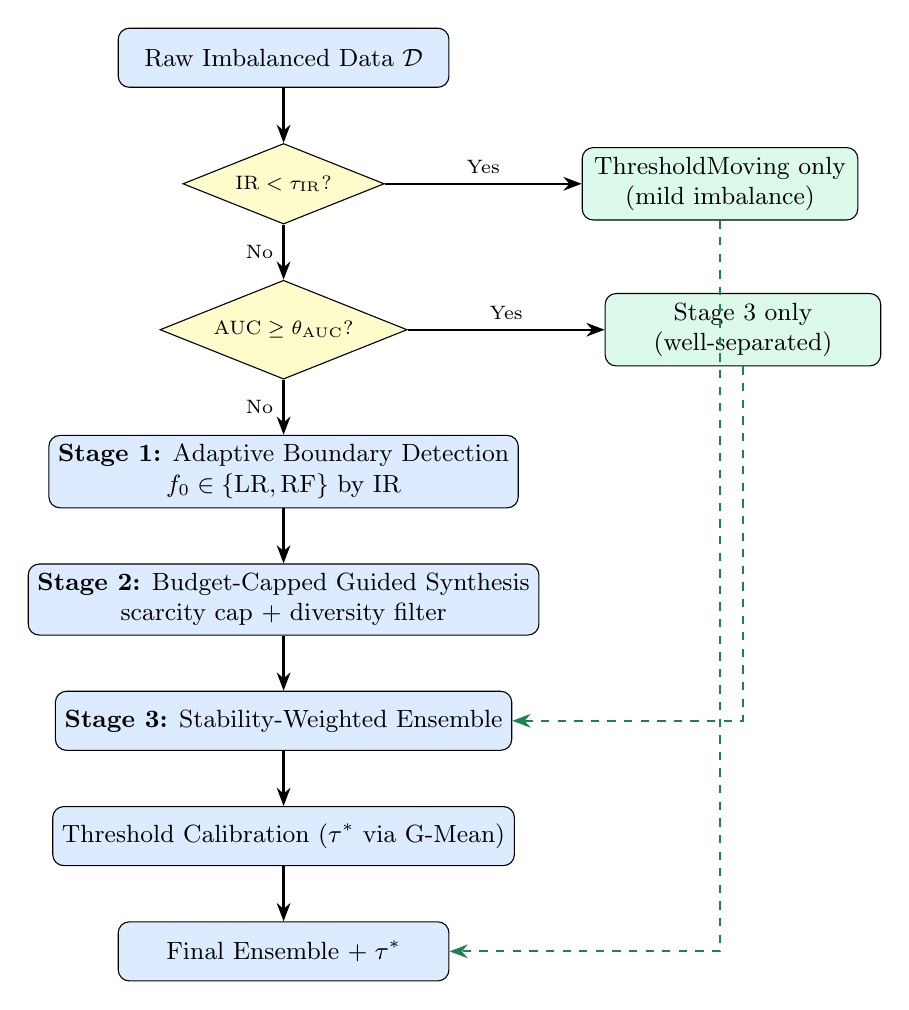
\begin{tikzpicture}[
    node distance=0.7cm and 1.2cm,
    box/.style={draw, rounded corners=4pt, fill=lightblue, minimum width=4.2cm, minimum height=0.75cm, align=center, font=\small},
    bypass/.style={draw, rounded corners=4pt, fill=lightgreen, minimum width=3.5cm, minimum height=0.65cm, align=center, font=\small},
    decision/.style={draw, diamond, fill=yellow!20, aspect=2.5, align=center, font=\scriptsize},
    arr/.style={-Stealth, thick},
    dasharr/.style={-Stealth, dashed, thick, color=accentgreen}
]

\node[box] (input) {Raw Imbalanced Data $\mathcal{D}$};
\node[decision, below=of input] (d1) {$\IR < \tau_{\IR}$?};
\node[bypass, right=2.5cm of d1] (bypass1) {ThresholdMoving only\\\small(mild imbalance)};
\node[decision, below=of d1] (d2) {$\mathrm{AUC} \ge \theta_{\mathrm{AUC}}$?};
\node[bypass, right=2.5cm of d2] (bypass2) {Stage 3 only\\\small(well-separated)};
\node[box, below=of d2] (s1) {\textbf{Stage 1:} Adaptive Boundary Detection\\$f_0 \in \{\mathrm{LR}, \mathrm{RF}\}$ by IR};
\node[box, below=of s1] (s2) {\textbf{Stage 2:} Budget-Capped Guided Synthesis\\scarcity cap $+$ diversity filter};
\node[box, below=of s2] (s3) {\textbf{Stage 3:} Stability-Weighted Ensemble};
\node[box, below=of s3] (cal) {Threshold Calibration ($\tau^*$ via G-Mean)};
\node[box, below=of cal] (out) {Final Ensemble $+\; \tau^*$};

\draw[arr] (input) -- (d1);
\draw[arr] (d1) -- node[left, font=\scriptsize]{No} (d2);
\draw[arr] (d1) -- node[above, font=\scriptsize]{Yes} (bypass1);
\draw[arr] (d2) -- node[left, font=\scriptsize]{No} (s1);
\draw[arr] (d2) -- node[above, font=\scriptsize]{Yes} (bypass2);
\draw[arr] (s1) -- (s2);
\draw[arr] (s2) -- (s3);
\draw[arr] (s3) -- (cal);
\draw[arr] (cal) -- (out);
\draw[dasharr] (bypass1) |- (out);
\draw[dasharr] (bypass2) |- (s3);

\end{tikzpicture}
\end{center}

\subsection{AMBA Pseudocode}

\begin{algorithm}[H]
\caption{AMBA: Adaptive Minority Boundary Augmentation}
\begin{algorithmic}[1]
\Require Dataset $\mathcal{D}$; hyperparameters $\tau_{\IR},\,\tau_{f_0},\,\tau_b,\,\alpha,\,\rho,\,\gamma,\,\delta,\,K,\,V,\,\theta_{\mathrm{AUC}}$
\Ensure Ensemble $\{(f_k, w_k)\}_{k=1}^K$; threshold $\tau^*$
\State \textbf{// ── Component 0: Adaptive Routing ──}
\State $\IR \leftarrow |\Dminus|/|\Dplus|$
\If{$\IR < \tau_{\IR}$}
  \State $f \leftarrow \text{CrossValidatedClassifier}(\mathcal{D})$
  \State $\tau^* \leftarrow \arg\max_\tau\,\mathrm{GMean}(P_f, \tau, \Dval)$
  \State \Return single classifier $f$ with threshold $\tau^*$
\EndIf
\State $\mathrm{AUC} \leftarrow$ 3-fold cross-validated AUC on $\mathcal{D}$
\State $\textit{augment} \leftarrow (\mathrm{AUC} < \theta_{\mathrm{AUC}})$
\If{$\textit{augment}$}
  \State \textbf{// ── Stage 1: Adaptive Boundary Detection ──}
  \If{$\IR \ge \tau_{f_0}$}
    \State $f_0 \leftarrow \text{RandomForest}(\text{max\_depth}=4,\,\mathcal{D})$; apply Platt scaling
    \State $\mathbf{g}_i \leftarrow \text{FiniteDiff}(\Pf, \mathbf{x}_i, \epsilon)$ for all $\mathbf{x}_i \in \Dplus$
  \Else
    \State $f_0 \leftarrow \text{LogisticRegression}(\mathcal{D})$
    \State $\mathbf{g}_i \leftarrow -\nabla_{\mathbf{x}}\Pf(y=1\mid\mathbf{x})\big|_{\mathbf{x}_i}$ for all $\mathbf{x}_i \in \Dplus$
  \EndIf
  \State $b_i \leftarrow 1 - 2|\Pf(y=1\mid\mathbf{x}_i) - 0.5|$ for all $\mathbf{x}_i \in \Dplus$
  \State $\Dbnd \leftarrow \{\mathbf{x}_i : b_i \ge \tau_b\}$;\; $\Dsafe \leftarrow \{\mathbf{x}_i : b_i < \tau_b\}$
  \State \textbf{// ── Stage 2: Budget-Capped Guided Synthesis ──}
  \State $n_{\mathrm{syn}} \leftarrow \min(n_{\mathrm{syn}},\,\lfloor\gamma\cdot|\Dplus|\rfloor)$\Comment{scarcity cap}
  \State $n^{\mathrm{bnd}} \leftarrow \lfloor\rho\cdot n_{\mathrm{syn}}\rfloor$;\; $n^{\mathrm{safe}} \leftarrow n_{\mathrm{syn}} - n^{\mathrm{bnd}}$
  \State $\mathcal{S}_{\mathrm{bnd}} \leftarrow \emptyset$
  \For{$n^{\mathrm{bnd}}$ iterations}
    \State Sample $\mathbf{x}_i \sim \Dbnd$;\; sample $\mathbf{x}_{\mathrm{nn}}$ from $k$-NN$(\mathbf{x}_i, \Dplus)$
    \State $\lambda_1, \lambda_2 \sim \mathcal{U}[0,1]$
    \State $\mathbf{x}_{\mathrm{syn}} \leftarrow \mathbf{x}_i + \lambda_1(\mathbf{x}_{\mathrm{nn}}-\mathbf{x}_i) + \alpha\lambda_2\hat{\mathbf{g}}_i$
    \If{$\min_j\|\mathbf{x}_{\mathrm{syn}} - \mathbf{x}_j\| \ge \delta$ for $\mathbf{x}_j \in \Dbnd$}\Comment{diversity filter}
      \State $\mathcal{S}_{\mathrm{bnd}} \leftarrow \mathcal{S}_{\mathrm{bnd}} \cup \{(\mathbf{x}_{\mathrm{syn}}, 1)\}$
    \EndIf
  \EndFor
  \State $\mathcal{S}_{\mathrm{safe}} \leftarrow \text{SMOTE}(\Dsafe,\,n^{\mathrm{safe}})$
  \State $\Daug \leftarrow \mathcal{D} \cup \mathcal{S}_{\mathrm{bnd}} \cup \mathcal{S}_{\mathrm{safe}}$
\Else
  \State $\Daug \leftarrow \mathcal{D}$\Comment{AUC-bypass: class-weighted, no augmentation}
\EndIf
\State \textbf{// ── Stage 3: Stability-Weighted Ensemble ──}
\For{$k = 1, \ldots, K$}
  \State $\mathcal{D}_k \leftarrow \text{Bootstrap}(\Daug)$;\; train $f_k$ on $\mathcal{D}_k$
  \State $r_k^{(1)}, \ldots, r_k^{(V)} \leftarrow V\text{-fold minority recall on } \Daug$
  \State $\sigma_k \leftarrow \mathrm{std}(r_k^{(1)}, \ldots, r_k^{(V)})$;\;
         $\tilde{w}_k \leftarrow 1/(1+\sigma_k)$
\EndFor
\State $w_k \leftarrow \tilde{w}_k / \sum_j \tilde{w}_j$ for all $k$
\State $\tau^* \leftarrow \arg\max_\tau\,\mathrm{GMean}(\sum_k w_k P_{f_k}(y=1\mid\mathbf{x}),\,\tau,\,\Dval)$
\State \Return $\{(f_k, w_k)\}_{k=1}^K,\;\tau^*$
\end{algorithmic}
\end{algorithm}

\subsection{Hyperparameters and Their Roles}

\begin{table}[ht]
\centering
\caption{AMBA hyperparameters, their roles, defaults, and search ranges.}
\begin{tabular}{llll}
\toprule
\textbf{Parameter} & \textbf{Role} & \textbf{Default} & \textbf{Search Range} \\
\midrule
$\tau_b$      & Boundary proximity threshold                     & 0.6         & $\{0.4, 0.5, 0.6, 0.7, 0.8\}$ \\
$\alpha$      & Gradient direction weight                         & 0.3         & $[0, 1]$ \\
$\rho$        & Boundary-region sample fraction                  & 0.7         & $[0.5, 0.9]$ \\
$K$           & Ensemble size                                     & 10          & $\{5, 10, 20\}$ \\
$V$           & Stability estimation folds                        & 5           & $\{3, 5, 10\}$ \\
$k$-NN        & SMOTE neighbourhood size                          & 5           & $\{3, 5, 7, 10\}$ \\
$\tau_{\IR}$  & IR threshold for pre-flight bypass               & 5           & $\{3, 5, 8, 10\}$ \\
$\tau_{f_0}$  & IR threshold for $f_0$ selector (LR $\to$ RF)    & 20          & $\{10, 20, 30, 50\}$ \\
$\epsilon$    & Finite-difference step size (RF gradients)        & $10^{-3}\bar{\sigma}$ & --- \\
$\gamma$      & Scarcity cap multiplier ($n_{\mathrm{syn}}^{\max} = \gamma|\Dplus|$) & 3.0 & $\{1.5, 2, 3, 5\}$ \\
$\delta$      & Min diversity distance                            & $0.01\bar{\sigma}$ & $\{0.001, 0.01, 0.05\}\bar{\sigma}$ \\
$\theta_{\mathrm{AUC}}$ & AUC threshold for Stage 2 bypass           & 0.97        & $\{0.95, 0.97, 0.99\}$ \\
\bottomrule
\end{tabular}
\end{table}

\subsection{What AMBA Does That Existing Methods Do Not}

\begin{table}[ht]
\centering
\caption{Qualitative comparison of AMBA against the existing baseline techniques.}
\begin{tabular}{lccccc}
\toprule
\textbf{Property} & \textbf{SMOTE} & \textbf{ADASYN} & \textbf{Class Wt.} & \textbf{EasyEns.} & \textbf{AMBA} \\
\midrule
Boundary-aware oversampling     & $\times$ & Partial  & $\times$ & $\times$ & $\checkmark$ \\
Gradient-directed synthesis     & $\times$ & $\times$ & $\times$ & $\times$ & $\checkmark$ \\
Stability-aware ensemble weights& $\times$ & $\times$ & $\times$ & $\times$ & $\checkmark$ \\
Ensemble aggregation            & $\times$ & $\times$ & $\times$ & $\checkmark$ & $\checkmark$ \\
Probability calibration         & $\times$ & $\times$ & Partial  & $\times$ & $\checkmark$ \\
IR-adaptive routing             & $\times$ & $\times$ & $\times$ & $\times$ & $\checkmark$ \\
Adaptive non-linear $f_0$       & $\times$ & $\times$ & $\times$ & $\times$ & $\checkmark$ \\
Scarcity-aware budget cap       & $\times$ & $\times$ & $\times$ & $\times$ & $\checkmark$ \\
Diversity filter                & $\times$ & $\times$ & $\times$ & $\times$ & $\checkmark$ \\
AUC-gated bypass                & $\times$ & $\times$ & $\times$ & $\times$ & $\checkmark$ \\
Model-agnostic                  & $\checkmark$ & $\checkmark$ & Partial & $\checkmark$ & $\checkmark$ \\
\bottomrule
\end{tabular}
\end{table}

% ════════════════════════════════════════════════════════════════════════════
\section{Experimental Roadmap}

\subsection{Experimental Design}

The study proceeds in five phases:

\begin{enumerate}[label=\textbf{Phase \arabic*.}, leftmargin=*, itemsep=4pt]
  \item \textbf{Data Preparation.} Loading, preprocessing, and stratified splitting.
  \item \textbf{Baseline Evaluation.} All seven models on raw imbalanced data; no correction.
  \item \textbf{Existing Technique Baselines.} Nine baseline techniques applied to every
        model--dataset combination.
  \item \textbf{AMBA Evaluation.} AMBA applied to all model--dataset combinations with
        nested cross-validation for hyperparameter tuning.
  \item \textbf{Stability and Comparative Analysis.} Stability profiles, technique--model
        interaction heatmaps, synthetic sample distribution visualisation, and failure mode
        characterisation.
\end{enumerate}

\subsection{Phase 1: Data Preparation}

Each dataset will be subjected to the following preprocessing steps:
\begin{itemize}[itemsep=2pt]
  \item Missing value imputation: median for continuous features, mode for categorical
  \item Feature scaling via \texttt{StandardScaler} (zero mean, unit variance)
  \item Stratified 5-fold cross-validation split (preserves per-fold class ratio)
  \item Held-out test set (20\,\% of data) reserved for final evaluation
\end{itemize}

\subsection{Phase 2: Baseline Evaluation}

All seven models are trained on the raw imbalanced data with no correction applied. All
metrics from Table~4 are recorded for each fold, establishing the unadjusted performance
floor from which improvements are measured.

\subsection{Phase 3: Existing Technique Baselines}

Each of the nine existing techniques is applied to every model--dataset combination. The
full result matrix comprises:
\[
  \underbrace{7}_{\text{models}} \times \underbrace{4}_{\text{datasets}} \times \underbrace{9}_{\text{techniques}} = 252 \text{ experiment cells}.
\]
Each cell reports the mean and CV for every metric.

\subsection{Phase 4: AMBA Evaluation}

AMBA is applied to all model--dataset combinations with hyperparameters tuned via nested
cross-validation to prevent data leakage. Each run uses $K = 10$ ensemble members and
$V = 5$ stability estimation folds. The routing components are engaged automatically based
on each dataset's IR and pilot AUC.

\subsection{Phase 5: Analysis}

Beyond aggregate tables, Phase 5 performs four targeted analyses:

\begin{enumerate}[itemsep=4pt]
  \item \textbf{Stability profiles.} Plot $\CV(\text{F1})$ as a function of IR for each model
        family. We expect a positive correlation between IR and instability that AMBA should
        consistently dampen.
  \item \textbf{Technique--model interaction.} Produce heatmaps of F1 improvement per
        technique per model to expose which pairings systematically favour or harm particular
        architectures.
  \item \textbf{Synthetic sample distribution.} Visualise AMBA-generated samples via PCA
        or $t$-SNE to verify that boundary-directed synthesis produces samples geometrically
        closer to the decision boundary than standard SMOTE, and that the diversity filter
        prevents clustering.
  \item \textbf{Routing analysis.} Characterise how often each routing path (IR-bypass,
        AUC-bypass, full pipeline) is triggered across model--dataset combinations, and
        whether the routing decisions correlate with performance outcomes.
\end{enumerate}

% ════════════════════════════════════════════════════════════════════════════
\section{Expected Contributions}

This study aims to make three distinct contributions to the imbalanced learning literature:

\begin{enumerate}[itemsep=6pt]
  \item \textbf{A systematic instability benchmark.} A publicly reproducible table of mean
        and CV metrics for 7 models $\times$ 4 datasets $\times$ 10 techniques
        (9 existing + AMBA). This alone fills a recognised gap in the literature.

  \item \textbf{A characterisation of model--imbalance interaction.} An empirical account of
        how model capacity, decision-boundary geometry, and imbalance ratio jointly determine
        prediction stability.

  \item \textbf{The AMBA framework.} A principled, model-agnostic technique that
        simultaneously addresses boundary coverage, prediction stability, and regime-adaptive
        routing, with clearly stated hyperparameters and complete pseudocode for
        reproducibility. AMBA is the first imbalance-handling framework to incorporate all
        of the following in a single coherent design: boundary-guided synthesis,
        gradient-directed interpolation, scarcity-proportional budget control, diversity
        filtering, stability-weighted ensemble aggregation, and adaptive IR/AUC routing.
\end{enumerate}

% ════════════════════════════════════════════════════════════════════════════
\section{Conclusion}

This document has laid out a complete research pitch for an empirical study of model
instability under minority data scarcity. We have identified four datasets spanning a wide
range of imbalance ratios, selected seven diverse classifiers, defined a dual-criterion
evaluation suite covering both performance and stability, catalogued existing techniques to
be used as baselines, and introduced AMBA---a novel four-component framework that
combines adaptive routing, boundary-guided synthetic oversampling with scarcity-proportional
budget control, and stability-weighted ensemble aggregation.

The core message is straightforward: mean F1-score is an incomplete picture. A technique
that halves prediction variance, even at a small cost to the mean, is often far more valuable
in any deployment context where reliable minority-class detection matters. Equally important
is the recognition that no single augmentation strategy is optimal across all imbalance
regimes: at mild imbalance, simple threshold calibration dominates; at extreme imbalance
with tiny minority counts, unconstrained synthesis causes mode collapse; when classes are
already well-separated, augmentation adds noise, not signal. AMBA is designed with both
principles as primary objectives---stability maximisation and regime-adaptive strategy
selection.

The next step is implementation and execution of the experimental roadmap described in
Section~8.

\vspace{1em}
\noindent\textit{This document is a research pitch. All claims about AMBA are
design-time hypotheses grounded in the motivation for each architectural decision.
No experimental results are reported.}

\end{document}